% This is samplepaper.tex, a sample chapter demonstrating the
% LLNCS macro package for Springer Computer Science proceedings;
% Version 2.20 of 2017/10/04
%
\documentclass[runningheads,a4paper]{llncs}
%
\usepackage{graphicx}
\usepackage[latin1]{inputenc}
\usepackage{amsmath, amssymb, amsfonts, dsfont, mathtools}
% Used for displaying a sample figure. If possible, figure files should
% be included in EPS format.
\usepackage{color}
\usepackage{multirow,array}%multicol
\usepackage [ all ]{xy}
\usepackage{pict2e,picture}
\usepackage{epsfig}
\usepackage{xcolor,tikz}
\usetikzlibrary{fit}
\usepackage{verbatim}
\usepackage[ruled,vlined,linesnumbered]{algorithm2e}
\usepackage{array}

\newcommand{\keywords}[1]{\par\addvspace\baselineskip
\noindent\keywordname\enspace\ignorespaces#1}

\usepackage{soul,hyperref}


\newcommand{\K}{\mathbb{K}}
\newcommand{\M}{\mathbb{M}}
\newcommand{\calC}{\mathcal C}
\newcommand{\calM}{\mathcal M}
\newcommand{\up}[1][]{{^{\uparrow_{#1}}}}
\newcommand{\down}[1][]{{^{\downarrow^{#1}}}}
\renewcommand{\emptyset}{\varnothing}
\newcommand{\obotSymbol}{%
	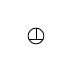
\begin{tikzpicture}[scale=0.1, line width=0.11mm]
		\draw (0,-0.5)--(0,1); \draw (-0.866,-0.5)--(0.866,-0.5);
		\draw (0,0) circle [radius=1];
\end{tikzpicture}}
\newcommand{\obot}{\mathbin{\raisebox{-0pt}{\obotSymbol}}}
\newcommand{\cupbotSymbol}{%
	\begin{tikzpicture}[scale=0.1, line width=0.11mm]
		\draw (0,-0.5) -- (0,1);
		\draw (-0.866,-0.5) -- (0.866,-0.5);
		\node[scale = 1] () at (0,0) {$\cup$};
\end{tikzpicture}}
\newcommand{\cupbot}{\mathbin{\raisebox{-2.5pt}{\cupbotSymbol}}}
\newcommand{\adjoint}{\mathop{\&}\nolimits}
\newcommand{\G}{\text{G}}
\renewcommand{\P}{\text{P}}
\let\oldLcommand\L
\let\L\relax
\def\L{\text{\oldLcommand}}

\newcommand{\editornote}[1]{{\normalfont \textcolor{red}{[#1]}}}
\newcounter{editorcommentcounter}
\newcommand{\editorcomment}[2][]{{%
	\normalfont
	\stepcounter{editorcommentcounter}%
	\textsuperscript{\textcolor{red}{(\arabic{editorcommentcounter})}}%
	\marginpar{\footnotesize\textcolor{red}{\arabic{editorcommentcounter}. #2}}%
}}



\newcommand{\cred}[1]{{\color{red} #1}}
\newcommand{\cb}[1]{{\color{blue}#1}}
\newcommand{\cy}[1]{{\color{cyan} #1}}
\newcommand{\cg}[1]{{\color{green!50!black} #1}}
%
\newcommand{\ct}[1]{\cred{\textst{#1}}}
\definecolor{naranjauca}{cmyk}{ 0, 0.6, 1, 0}
%\xdefinecolor{naranjauca}{rgb}{1, 0.45, 0}
\newcommand{\cn}[1]{{\color{naranjauca} #1}}
\def\seealso#1{\mbox{}%
	\marginpar[\raggedleft $\rightarrow$\\ \small \cn{#1}]%
	{\raggedright $\leftarrow$\small \cn{#1}}\ignorespaces}

\def\seealsob#1{\mbox{}%
	\marginpar[\raggedleft $\rightarrow$\\ \small {#1}]%
	{\raggedright $\leftarrow$\small {#1}}\ignorespaces}
% If you use the hyperref package, please uncomment the following line
% to display URLs in blue roman font according to Springer's eBook style:
\renewcommand\UrlFont{\color{blue}\rmfamily}

\begin{document}
	
\mainmatter  % start of an individual contribution

%
%\title{The notion of bond in the\\ multi-adjoint concept lattice framework\thanks{Partially supported by the the 2014-2020 ERDF Operational Programme in collaboration with the State Research Agency (AEI) in project PID2019-108991GB-I00, and with the Department of Economy, Knowledge, Business and University of the Regional Government of Andalusia in project FEDER-UCA18-108612, and by the European Cooperation in Science \& Technology (COST) Action CA17124.}}
%
\title{The notion of bond in the\\ multi-adjoint concept lattice framework}
\titlerunning{}
%Factorization of multi-adjoint contexts based on thresholds}
% If the paper title is too long for the running head, you can set
% an abbreviated paper title here
%
\author{}
\institute{}
%\author{Roberto G. Arag\'on%\orcidID{0000-0002-8927-5945} 
%\and
%Jes\'us Medina%\orcidID{0000-0002-3931-5873} 
%\and
%Samuel Molina-Ruiz%\orcidID{}
%}
%
%\authorrunning{R.G. Arag\'on, J. Medina, S. Molina-Ruiz}
% First names are abbreviated in the running head.
% If there are more than two authors, 'et al.' is used.
%
%\institute{Department of Mathematics, University of C\'adiz, Spain
%\email{\{roberto.aragon,jesus.medina,samuel.molina\}@uca.es}}
%
\maketitle              % typeset the header of the contribution
% 
\begin{abstract}

The notion of bond in formal concept analysis arose as a mechanism for aggregating contexts, preserving the main information of the original ones. 
This notion can also be fundamental in the inverse process, that is, in the factorization of contexts, which will allow the computation of the information of a real context from smaller subcontexts (distributed computing). 
This paper considers the flexible fuzzy multi-adjoint framework in order to introduce the first definition of bond in this setting and presents the first properties and examples of this definition. 
	
\keywords{Formal concept analysis, bonds, multi-adjoint framework.}
\end{abstract}

\section{Introduction}

Ability to efficiently process large amounts of data  is essential for extracting useful information from many of the existing real databases. Formal concept analysis (FCA) is a relevant mathematical theory for extracting knowledge from relational databases since its introduction in the eighties~\cite{Wille:1982}. The theory deems databases as formal contexts~\cite{GanterW}, that is, as a triple interpreted as a relation/table between   a set of objects and a set of attributes. FCA tools are capable of manipulating data and extracting relevant information, which is represented using the algebraic structure of a complete lattice~\cite{GanterW}.  Several extensions of this mathematical theory have been introduced in a fuzzy environment~\cite{belohlavek:2001,burusco:1998,Stano:GCL}, and theoretical~\cite{aragonMath21,aragonJCAM21,OJEDAHERNANDEZ23,PEREZGAMEZ2023505} and applied~\cite{Alcalde2020Red,alilipedrycz2023,SOKOL2023108940} {advances} are made on a daily basis. Among the existing fuzzy extensions,  the multi-adjoint framework~\cite{TFS:2020-acmr,ar:ins:2015,ins2018:cmr,mor-fss-cmpi} is one of the most flexible and versatile, making it ideal for modeling real-world problems.

Various methods have been developed and utilized in FCA to simplify data processing, %~\cite{bmrd:FCARST:f,Cornejo2017},
such as factoring and aggregating data tables~\cite{COAMfac2024,BELOHLAVEK20103,dubois:2012,KRIDLO22IS,valverdeipmu18art}. These techniques enable the reduction of large tables into smaller ones, known as factors, from which important information can be extracted. In addition, these factors can be aggregated without modifying the information present in them. In particular, we focus on the notion of bond between formal contexts, which was originally defined in the classical setting~\cite{GanterW} and was extended to the fuzzy framework using residuated lattices~\cite{konecnyijgs16,KridloKO12,KRIDLO2023119498}. Bonds allow the aggregation of contexts while preserving the information contained in the concepts generated by each individual context. This work aims to extend the aforementioned notion to the multi-adjoint framework and to analyze the conditions that enable obtaining bonds in a simpler manner.

The paper will introduce in Section~\ref{sec:preliminaries} diverse preliminary notions in FCA, including the crisp notion of bond. In Section~\ref{sec:multi-adjoint}, the definition of bond in the multi-adjoint concept lattice framework will be presented based on  intents of fuzzy objects and extents of fuzzy attributes of the given context. Furthermore, an illustrative example  will be included to display particular cases of bonds and    relations that are not  bonds.  This section will also  be focused on two  notable fuzzy  relations: the constantly top and constantly bottom relations, showing that the first is always a bond and  introducing a sufficient condition  to ensure that the second is a bond. This result will also be illustrated with examples. The paper will finish with diverse conclusions and  prospects of future works.

\section{Preliminaries}\label{sec:preliminaries}

In this preliminaries section, we introduce foundational notions related to FCA. Throughout this paper, the notation $A^B$ will be employed to denote maps from $B$ to $A$. Particularly, if $A = \{1, \dots, n\}$ we may use $n^B$ to denote $\{1, \dots, n\}^B$. In addition, if a map $f \colon A \to B$ takes only one value, $b \in B$, we may write it as $f \equiv b$. 

We now proceed to define what precisely a context is within the setting of FCA.

\begin{definition}

A \emph{context} is a tuple $(O, P, R)$ such that $O$ and $P$ are non-empty sets (usually interpreted as objects and properties, respectively) and $R$ is a relation in $O \times P$.

\end{definition}

In addition, the derivation operators $\up \colon 2^O \to 2^P$ and $\down \colon 2^P \to 2^O$ are defined, for all $X \subseteq O$ and $A \subseteq P$, as
\begin{align*}
	X\up &= \{a \in P \mid (x, a) \in R, \text{ for all $x \in X$}\} \\
	A\down &= \{x \in O \mid (x, a) \in R, \text{ for all $a \in A$}\}
\end{align*}

A \emph{concept} is a pair $\langle X, A \rangle$ satisfying that $X\up = A$ and $A\down = X$, where $X$ is called the \emph{extent} and $A$ is called the \emph{intent}. %\cred{The set of all the concepts of the context $(O, P, R)$ is denoted by $\calC(O, P, R)$, and with the ordering defined by $\langle X_1, A_1 \rangle \preceq \langle X_2, A_2 \rangle$ if and only if $X_1 \subseteq X_2$ (equivalently $A_2 \subseteq A_1$), for all $\langle X_1, A_1 \rangle, \langle X_2, A_2 \rangle \in \calC(O, P, R)$, forms a complete lattice~\cite{DaveyPriestley} called \emph{concept lattice}.}

% \color{red}
% Additionally, we introduce the notion of a closed relation:

% \begin{definition}
	
% Let $(O, P, R)$ be a context. A subrelation $R' \subseteq R$ is a \emph{closed relation} of the context $(O, P, R)$ if every concept of the context $(O, P, R')$ is also a concept of $(O, P, R)$.

% \end{definition}

% One way to recognize when a relation is closed is given by the following characterization.

% \begin{proposition}\label{prop:characterization-of-bonds}
	
% The closed relations of a context $(O, P, R)$ are precisely those subrelations $R' \subseteq R$ which satisfy the following condition:
% \begin{center}\begin{minipage}{0.9\textwidth}
% 	$(x, a) \in R \setminus R'$ implies $(y, a) \notin R$ for some $y \in O$ with $x\up[R'] \subseteq y\up[R']$ as well as $(x, b) \notin R$ for some $b \in P$ with $p\down[R'] \subseteq b\down[R']$.
% \end{minipage}\end{center}

% \end{proposition}

% The closed relations characterize the complete sublattices of a concept lattice, as shown in the next result.

% \begin{theorem}
	
% If $R'$ is a closed relation of the context $(O, P, R)$, then $\calC(O, P, R')$ is a complete sublattice of $\calC(O, P, R)$, with
% \[
% R' = \bigcup \{X \times A \mid (X, A) \in \calC(O, P, R)\}
% \]
% Inversely, for every complete sublattice $U$ of $\calC(O, P, R)$, the relation
% \[
% R' = \bigcup \{X \times A \mid (X, A) \in U\}
% \]
% is a closed relation of $(O, P, R)$ with $\calC(O, P, R') = U$.

% \end{theorem}

% As explained in the introduction, our focus is on joining a family of contexts. The natural environment for this is the direct, or cartesian, product of concept lattices. We want to study the complete sublattices of this product that preserve the original concept lattices. With this idea in mind, we introduce the notion of a subdirect product.

% \begin{definition}
	
% A \emph{subdirect product} of complete lattices is a complete sublattice of the direct product for which the canonical projections onto the factors is surjective.

% \end{definition}

% In order to work with this notion, we are going to define the direct sum of contexts.

% \begin{definition}
	
% Let $\Lambda$ be an arbitrary set of indices. Given a family $\{\K_i = (O_i, P_i, R_i)\}_{i \in \Lambda}$ of disjoint contexts\footnote{Two contexts $(O_1, P_1, R_1)$ and $(O_2, P_2, R_2)$ are disjoint if $O_1 \cap O_2 = P_1 \cap P_2 = \emptyset$}, we define their \emph{direct sum} as the context $\sum_{i \in \Lambda} \K_i = (O_\Lambda, P_\Lambda, R_\Lambda)$ where\editorcomment{hay un abuso de notación puesto que se usa $\Lambda$, como conjunto de índices y como subíndice (notación). Tendríamos que comentarlo.}
% \[
% O_\Lambda = \bigcup_{i \in \Lambda} O_i, \quad P_\Lambda = \bigcup_{i \in \Lambda} P_i, \quad R_\Lambda = \bigcup_{i \in \Lambda} R_i \cup \bigcup_{j \neq i} (O_j \times P_j).
% \]

% \end{definition}

% The direct sum is a more natural way to work with the direct product of the concept lattices, but it is equivalent thanks to the following theorem.

% \begin{theorem}\label{th:isomorphism-sum-context-lattice---prod-concept-lattice}
	
% The concept lattice of a direct sum of context is isomorphic to the cartesian product of the concept lattice of the factors, that is,
% \[
% \calC ( \sum_{i \in \Lambda} \K_i ) \cong \bigtimes_{i \in \Lambda} \calC(\K_i).
% \]
% The map $\mathfrak C \colon \calC ( \sum_{i \in \Lambda} \K_i ) \to \bigtimes_{i \in \Lambda} \calC(\K_i)$ given by
% \[
% \mathfrak C (X, A) = (X \cap O_i, A \cap P_i)_{i \in \Lambda}, \quad \text{for all $\textstyle(X, A) \in \calC(\sum_{i \in \Lambda} \K_i)$}
% \]
% is a natural isomorphism. Moreover, the canonical projection together with this isomorphism is the map $\pi_i \colon \calC (\sum_{i \in \Lambda} \K_i) \to \calC(\K_i)$ given by 
% \[
% \pi_i(X, A) = (X \cap O_i, A \cap P_i), \quad \text{for all $\textstyle (X, A) \in \calC ( \sum_{i \in \Lambda} \K_i )$}.
% \]

% \end{theorem}

% We end this introduction showing how subdirect products and direct sums relate. This relation lets us use the more natural notion of direct sum in order to join different contexts.

% \begin{proposition}\label{prop:subdirec-products-characterization}
	
% The subdirect product of the concept lattices $\calC(\K_i)$ are one to one with the closed relations $R$ of the sum context $\sum_{i \in \Lambda} \K_i$ with $R \cap (O_i \times P_i) = R_i$ for all $i \in \Lambda$.

% \end{proposition}
% color{black}

%\section{Bonds}\label{sec:bonds}

%since the aim of this work is to investigate methods for aggregating contexts (factors) and constructing a new context from them. This new context has to preserve the information contained in the factors.  we will pursue this idea presenting the theory of bonds in the classical case and working through an example. In Section~\ref{sec:multi-adjoint}, we will translate these notions into the multi-adjoint framework.

From now on, we will consider a family of contexts $\{(O_i, P_i, R_i)\}_{i \in \Gamma}$, with $\Gamma$ a non-empty set of indices. We will simply denote the derivation operators $\up$ and $\down$ in each context $(O_i, P_i, R_i)$ as $\up[i]$ and $\down[i]$, respectively. Moreover, if $R_{ij} \subseteq O_i \times P_j$ is a relation, we define the mappings $\up[ij] \colon 2^{O_i} \to 2^{P_j}$ and $\down[ij] \colon 2^{P_j} \to 2^{O_i}$ as
\begin{align*}
	X\up[ij] &= \{a \in P_j \mid (x, a) \in R_{ij}, \text{ for all $x \in X$}\} \\
	A\down[ij] &= \{x \in O_i \mid (x, a) \in R_{ij}, \text{ for all $a \in A$}\}
\end{align*}
for all $X \subseteq O_i$ and $A \subseteq P_j$. When we consider $X = \{x\}$ and $A = \{a\}$, we may use the notation $x\up[ij]$ and $a\down[ij]$ instead of $\{x\}\up[ij]$ and $\{a\}\down[ij]$.

Next, the notion of bond is introduced as a method of aggregating contexts (factors). Bonds allow to construct a new context from factors while preserving the information they contain. In Section~\ref{sec:multi-adjoint}, we will translate this notion into the multi-adjoint framework.
%Our initial step will involve defining the concept of a bond.

\begin{definition}\label{def:bond}

Given two different contexts $(O_i, P_i, R_i)$ and $(O_j, P_j, R_j)$, a \emph{bond} from $(O_i, P_i, R_i)$ to $(O_j, P_j, R_j)$ is a relation $R_{ij} \subseteq O_i \times P_j$ such that
\begin{itemize}
	\item $x\up[ij]$ is an intent of $(O_j, P_j, R_j)$ for every object $x \in O_i$,
	\item $a\down[ij]$ is an extent of $(O_i, P_i, R_i)$ for every property $a \in P_j$.
\end{itemize}

\end{definition}

Now, we will examine this definition more closely through a practical example

\begin{example}\label{ex:crisp-bonds}

Consider two contexts $(O_1, P_1, R_1)$ and $(O_2, P_2, R_2)$ where
\begin{align*}
	O_1 &= \{x_1, x_2\}, & P_1 &= \{a_1, a_2\}, & R_1 &= \{(x_1, a_1), (x_1, a_2), (x_2, a_2)\} \\
	O_2 &= \{x_3, x_4\}, & P_2 &= \{a_3, a_4\}, & R_2 &= \{(x_3, a_3), (x_4, a_4)\}
\end{align*}
A bond can be visualized by placing the two contexts diagonally, one beneath the other, and the bond in the top right corner (a bond $R_{ji}$ from $(O_j, P_j, R_j)$ to $(O_i, P_i, R_i)$ would be placed in the bottom left), as observed in Table~\ref{tab:example-crisp-bonds}. 
Since the set of objects and the set of properties are always an extent and an intent of a context, we are guaranteed that the relation $R_{1\,2}^\top = O_1 \times P_2$ is a bond. Indeed, for any $x \in O_1$, $x\up[1\,2] = P_2$ is an intent of $(O_2, P_2, R_2)$ and, for any $a \in P_2$, $a\down[1\,2] = O_1$ is an extent of $(O_1, P_1, R_1)$.

\begin{table}[h!]
	\centering
	\begin{tabular}{w{c}{15pt} || w{c}{15pt} | w{c}{15pt} || w{c}{15pt} | w{c}{15pt}}
		& $a_1$ & $a_2$ & $a_3$ & $a_4$ \\\hline\hline
		$x_1$ & $\times$ & $\times$ & $\times$ & $\times$ \\\hline
		$x_2$ & & $\times$ & $\times$ & \\\hline\hline
		$x_3$ & & & $\times$ & \\\hline
		$x_4$ & & & & $\times$\\
	\end{tabular}
	\begin{tikzpicture}[overlay, remember picture]
		\draw[black, ultra thick] (-1.38,-0.12) rectangle (-0.11,0.68);
		\node[right] () at (-0.11,0.28) {$R_{1\,2}^1$};
		% \draw (-1.38,-0.12) circle (0.02);
		% \draw (-0.11,0.68) circle (0.02);
	\end{tikzpicture}
	\hspace{1cm}
	\begin{tabular}{w{c}{15pt} || w{c}{15pt} | w{c}{15pt} ||
	w{c}{15pt} | w{c}{15pt}} & $a_1$ & $a_2$ & $a_3$ & $a_4$ \\\hline\hline
	$x_1$ & $\times$ & $\times$ & & \\\hline 
	$x_2$ & & $\times$ &$\times$ & \\\hline\hline 
	$x_3$ & & & $\times$ & \\\hline
	 $x_4$ & & & &	$\times$\\
	 \end{tabular}
	\begin{tikzpicture}[overlay, remember picture]
		\draw[black, ultra thick] (-1.38,-0.12) rectangle (-0.11,0.68);
		\node[right] () at (-0.11,0.28) {$R_{1\,2}^2$};
		% \draw (-1.38,-0.12) circle (0.02);
		% \draw (-0.11,0.68) circle (0.02);
	\end{tikzpicture}
   \vspace{1ex}
	\caption{
    {Tables showing the relations $R_1$ and $R_2$ of Example~\ref{ex:crisp-bonds} together with $R_{1\,2}^1$ (left table) and $R_{1\,2}^2$ (right table).}
    % Tables showing the contexts $(O_1, P_1, R_1)$ and $(O_2, P_2, R_2)$ on the diagonal and the relations $R_{1\,2}^1$ (left table) and $R_{1\,2}^2$ (right table) of Example~\ref{ex:crisp-bonds} on the top right corner.
    }
	\label{tab:example-crisp-bonds}
 \vspace*{-2em}
\end{table}

We can usually find other non-trivial bonds, such as%$R_{1\,2}^1 = \{(x_1, a_3), (x_1, a_4), (x_2, a_3)\}$
\[
R_{1\,2}^1 = \{(x_1, a_3), (x_1, a_4), (x_2, a_3)\}
\]
For this relation, $x_1\up[1\,2] = \{a_3, a_4\}$ and $x_2\up[1\,2] = \{a_3\}$ are intents of $(O_2, P_2, R_2)$. The first one because it is the set of properties $P_2$ and the second one because
\[
a_3\down[2]\up[2] = x_3\up[2] = \{a_3\}
\]
Likewise, $a_3\down[1\,2] = \{x_1, x_2\}$ and $a_4\down[1\,2] = \{x_1\}$ are extents of $(O_1, P_1, R_1)$, the first one for being the set of objects $O_1$ and the second one because
\[
x_1\up[1]\down[1] = \{a_1, a_2\}\down[1] = \{x_1\}
\]

However, not all relations in $O_1 \times P_2$ are bonds. Consider for instance the relation $R_{1\,2}^2 = \{(x_2, a_3)\}$. This relation is not a bond because $a_3\down[1\,2] = \{x_2\}$ is not an extent of $(O_1, P_1, R_1)$, that is, 
\[
x_2\up[1]\down[1] = a_2\down[1] = \{x_1, x_2\} \neq \{x_2\}
\]

Another interesting case is the empty relation, $R_{1\,2}^\bot = \emptyset$. In this case, the relation $R_{1\,2}^\bot$ is not a bond from $(O_1, P_1, R_1)$ to $(O_2, P_2, R_2)$ due to
\[
\varnothing\up[1]\down[1] = \{a_1, a_2\}\down[1] = \{x_1\} \neq \varnothing
\]
This means that the empty set is not an extent of $(O_1, P_1, R_1)$. \qed
% \begin{figure}
% 	\centering
% 	\includegraphics[height = 0.2\textwidth]{im/ex-crisp-K1.png}
% 	\hspace{1cm}
% 	\includegraphics[height = 0.2\textwidth]{im/ex-crisp-K2.png}
% 	\hspace{1cm}
% 	\includegraphics[height = 0.2\textwidth]{im/ex-crisp-R12^top.png}
% 	\hspace{1cm}
% 	\includegraphics[height = 0.2\textwidth]{im/ex-crisp-R12^1.png}
% 	\caption{From left to right: the concept lattices for $\K_1$, $\K_2$, $(O_1, P_2, R_{1\,2}^\top)$, $(O_1, P_2, R_{1\,2}^1)$ and $(O_1, P_2, R_{1\,2}^1 \cup R_{1\,2}^\top)$\editornote{not right.}.}
% \end{figure}

\end{example}

\begin{remark}\label{rem:bottom-bond-crisp}
As Example~\ref{ex:crisp-bonds} shows, the empty relation is not always an extent or intent of a context and, therefore, it is not a bond. However, there are cases where it is actually a bond. Given two different contexts $(O_i, P_i, R_i)$ and $(O_j, P_j, R_j)$ satisfying that for every object $x \in O_i$, there exists $a \in P_i$ such that $(x, a) \notin R_i$, and for every property $a' \in P_j$, there exists $x' \in O_j$ such that $(x', a') \notin R_j$, {then} the empty set is both an extent of $(O_i, P_i, R_i)$ and an intent of $(O_j, P_j, R_j)$. Therefore, these conditions guarantee that the relation $R_{ij}^\bot$ is a bond from $(O_i, P_i, R_i)$ to $(O_j, P_j, R_j)$.
%Given two contexts $(O_i, P_i, R_i)$ and $(O_j, P_j, R_j)$, the empty relation is not always a bond from $(O_i, P_i, R_i)$ to $(O_i, P_i, R_i)$ because the empty set is not always an extent or intent of a context. However, there are cases where it is actually a bond. If the contexts $(O_i, P_i, R_i)$ and $(O_i, P_i, R_i)$ satisfy that for every object $x \in O_i$ and property $a' \in P_j$, there exists $a \in P_i$ and $x' \in O_j$ such that $(x, a) \notin R_i$ and $(x', a') \notin R_j$, then this guarantees that the empty set is both an extent of $(O_i, P_i, R_i)$ and an intent of $(O_i, P_i, R_i)$ and therefore the relation $R_{ij}^\bot$ is a bond from $(O_i, P_i, R_i)$ to $(O_i, P_i, R_i)$.

\end{remark}

\section{Bonds on a multi-adjoint framework}\label{sec:multi-adjoint}

In the previous section, we dealt with the classical case, but when considering the fuzzy scenario, we need to work with a more general notion of context, where an object can have a truth degree value about whether it has a given attribute. In particular, we need to recall the fundamentals of the multi-adjoint framework in order to define a bonds between contexts associated with a multi-adjoint frame.
%In this section, we will recall the notion of a multi-adjoint framework and concept in order to define a bond between contexts associated to a multi-adjoint framework.

First, let us remember what a multi-adjoint framework is.

\begin{definition}
	
A \emph{multi-adjoint framework} is a tuple $(L_1, L_2, Q, \adjoint_1, \dots, \adjoint_n)$ where {$(L_1, \preceq_1, \bot_1, \top_1)$ and $(L_2, \preceq_2, \bot_2, \top_2)$} are complete lattices, $(Q, \leq)$ is a poset and $(\adjoint_k, \swarrow^k, \nwarrow_k)$ is an adjoint triple with respect to $L_1$, $L_2$ and $Q$, for all $k \in \{1, \dots, n\}$.

\end{definition}

Throughout this section, a multi-adjoint framework $(L_1, L_2, Q, \adjoint_1, \dots, \adjoint_n)$ will be fixed.
% \cb{, where $(L_1,\preceq_1,\bot_1,\top_1)$ and $(L_2,\preceq_2,\bot_2,\top_2)$}.
% \cred{We will denote the top and bottom elements of $L_1$ and $L_2$ as $\top_1$, $\bot_1$, $\top_2$ and $\top_2$, respectively.}
%The definition of a context is defined in the same way as the classical, adding a function which designates an adjoint triple to each pair of objects and properties. This notion is formalized in the following definition.
Once a multi-adjoint frame has been fixed, the notion of a context in that frame is defined in the following way.

\begin{definition}
	
A \emph{context} is a tuple $(O, P, R, \sigma)$, where $O$ is the set of objects, $P$ is the set of properties, $R$ is a $Q$-fuzzy relation $R \colon O \times P \to Q$ and $\sigma \colon O \times P \to \{1, \dots, n\}$ is a mapping which associates {each element in $O \times P$ with a specific adjoint triple.}
%\cred{a specific adjoint triple in the frame with any element in $O \times P$.}

\end{definition}

The extension of the concept-forming operators are the mappings $\up \colon L_1^O \to L_2^P$ and $\down \colon L_2^P \to L_1^O$ defined as:
\begin{align*}
	g\up(a) &= \inf \{R(x, a) \swarrow^{\sigma(x, a)} g(x) \mid x \in O\} \\
	f\down(x) &= \inf \{R(x, a) \nwarrow_{\sigma(x, a)} f(x) \mid a \in P\}
\end{align*}
for all $g \in L_1^O$, $f \in L_2^P$ and $a \in P$, $x \in O$. Equivalently, a pair $\langle g, f \rangle$ is called a \emph{multi-adjoint concept} if equalities $g\up = f$ and $f\down = g$ hold. %Similar to the classical case, the set of all concepts constitutes a complete lattice~\cite{mor-fss-cmpi}, called multi-adjoint concept lattice and denoted by $\calM$, under the order defined by $\langle g_1, f_1 \rangle \preceq \langle g_2, f_2 \rangle$ if and only if $g_1 \preceq_1 g_2$ as $L_1$-fuzzy sets (equivalently, $f_2 \preceq_2 f_1$), for all $\langle g_1, f_1 \rangle, \langle g_2, f_2 \rangle \in \calM$.

In addition, the following notion is related to a specific family of fuzzy subsets of $L_1^P$ that will play a fundamental role in this work.

\begin{definition}\label{fuzzy-attribute}

For each $a\in P$, the fuzzy subsets of attributes $\phi_{a,x}\in L_1^P$ defined, for all $x\in L_1$, as
$$ \phi_{a,x}(a') = \begin{cases}
 x& \hbox{if } a' = a\\
 \bot_1 &\hbox{if } a'\neq a
\end{cases}
$$
will be called \emph{fuzzy-attributes}.

\end{definition}

Analogously, the fuzzy-objects are defined in the same way.

Now, we are ready to establish the basis for defining a bond. Hereon, a family of contexts associated with the frame, $\{(O_i, P_i, R_i, \sigma_i)\}_{i \in \Gamma}$, will be considered. Given a $Q$-fuzzy relation $R_{ij}$ in $O_i \times P_j$ and $\sigma_{ij} \colon O_i \times P_j \to \{1, \dots, n\}$, we define the mappings $\up[ij] \colon L_2^{O_i} \to L_1^{P_j}$ and $\down[ij] \colon L_1^{P_j} \to L_2^{O_i}$ as
\begin{align*}
	g\up[ij](a) &= \inf \{R_{ij}(x, a) \swarrow^{\sigma_{ij}(x,a)} g(x) \mid x \in O_i\} \\
	f\down[ij](x) &= \inf \{R_{ij}(x, a) \nwarrow_{\sigma_{ij}(x,a)} f(a) \mid a \in P_j\}
\end{align*}
for each $g \in L_2^{O_i}$, $f \in L_1^{P_j}$ and $a \in P_j$, $x \in O_i$. Note that when we refer to the context $(O_i, P_i, R_i, \sigma_i)$, we will simply denote the concept-forming operators $\up$ and $\down$ as $\up[i]$ and $\down[i]$, respectively.

In Definition~\ref{def:bond}, we described a bond from $(O_i, P_i, R_i)$ to $(O_j, P_j, R_j)$ as a relation $R_{ij}$ in $O_i \times P_j$, which can also be interpreted as a new context $(O_i, P_j, R_{ij})$. This point of view is fundamental in the following definition of a bond between contexts associated with a multi-adjoint framework.

\begin{definition}
	
Given two different contexts $(O_i, P_i, R_i, \sigma_i)$ and $(O_j, P_j, R_j, \sigma_j)$, a \emph{multi-adjoint bond} from $(O_i, P_i, R_i, \sigma_i)$ to $(O_j, P_j, R_j, \sigma_j)$ is a context\\ $(O_i, P_j, R_{ij}, \sigma_{ij})$ such that $R_{ij} \subseteq O_i \times P_j$ and $\sigma_{ij} \colon O_i \times P_j \to \{1, \dots, n\}$ satisfying that
\begin{itemize}
	\item $\phi_{x,t}\up[ij]$ is an intent of $(O_j, P_j, R_j, \sigma_j)$, for every object $x \in O_i$,\\[-5pt]
	\item $\phi_{a,s}\down[ij]$ is an extent of $(O_i, P_i, R_i, \sigma_i)$, for every property $a \in P_j$,
\end{itemize}
where $s \in L_1$ and $t \in L_2$.

\end{definition}

{Henceforth, we will assume that $Q$ is bounded by a top element $\top_3$ and a bottom element $\bot_3$.} We are particularly interested in studying the contexts whose relations are all $\top_3$ or $\bot_3$, that is, $R_{ij}(x, a) = \top_3$, for all $(x, a) \in O_i \times P_j$, or $R_{ij}(x, a) = \bot_3$, for all $(x, a) \in O_i \times P_j$. We will simply denote these particular relations as $R_{ij}^\top$ and $R_{ij}^\bot$, respectively. 
Similar to the classical case, the former will always be a multi-adjoint bond, but the latter requires further study. Let us show this fact through an example.

\begin{example}\label{ex:multiadjoint-bonds}

Consider the multi-adjoint framework $([0, 1]_4, [0, 1]_4, [0, 1]_4, \adjoint^*_\G, \adjoint^*_\L)$ where $\adjoint^*_\G$ and $\adjoint^*_\L$ are the discretization of the G\"{o}del and \L ukasiewicz conjunctors, respectively. Also consider the contexts $(O_1, P_1, R_1, \sigma_1)$ and $(O_2, P_2, R_2, \sigma_2)$, where the relations $R_1$, $R_2$ and the maps $\sigma_1$, $\sigma_2$ are defined in Table~\ref{tab:example1-multiadjoint-bonds-R1-R2}.
%\cred{are defined in Table~\ref{tab:example1-multiadjoint-bonds-R1-R2}. and $\sigma_1(x, a) = \adjoint^*_\G$, for all $(x, a) \in O_1 \times P_1$ and $\sigma_2(x', a') = \adjoint^*_\L$, for all $(x', a') \in O_2 \times P_2$.}
\begin{table}[h]
	\centering
	\vspace{-1ex}
	% \begin{minipage}{0.25\textwidth}
	\begin{tabular}{w{c}{20pt} || w{c}{20pt} | w{c}{20pt}}
		$R_1$ & $a_1$ & $a_2$ \\\hline\hline
		$x_1$ & $0.5$ & $0.75$ \\\hline
		$x_2$ & $0.25$ & $1$
	\end{tabular}
    \hfill
	\begin{tabular}{w{c}{20pt} || w{c}{20pt} | w{c}{20pt}}
		$\sigma_1$ & $a_1$ & $a_2$ \\\hline\hline
		$x_1$ & $\adjoint^*_\G$ & $\adjoint^*_\G$ \\\hline
		$x_2$ & $\adjoint^*_\G$ & $\adjoint^*_\G$
	\end{tabular}
	% \end{minipage}
	% \begin{minipage}{0.2\textwidth}
	% 	\includegraphics[scale = 0.3]{im/ex-ma2-R1.png}
	% \end{minipage}
    \hfill
	% \begin{minipage}{0.25\textwidth}
	\begin{tabular}{w{c}{20pt} || w{c}{20pt} | w{c}{20pt}}
		$R_2$ & $a_3$ & $a_4$ \\\hline\hline
		$x_3$ & $1$ & $0.75$ \\\hline
		$x_4$ & $0.75$ & $1$
	\end{tabular}
    \hfill
	\begin{tabular}{w{c}{20pt} || w{c}{20pt} | w{c}{20pt}}
		$\sigma_2$ & $a_3$ & $a_4$ \\\hline\hline
		$x_3$ & $\adjoint^*_\L$ & $\adjoint^*_\L$ \\\hline
		$x_4$ & $\adjoint^*_\L$ & $\adjoint^*_\L$
	\end{tabular}
	% \end{minipage}
	% \begin{minipage}{0.2\textwidth}
	% 	\includegraphics[scale = 0.3]{im/ex-ma2-R2.png}
	% \end{minipage}
 \vspace{1ex}
	\caption{The relations $R_1$, $R_2$ and maps $\sigma_1$, $\sigma_2$ of the contexts $(O_1, P_1, R_1, \sigma_1)$ and $(O_2, P_2, R_2, \sigma_2)$ in Example~\ref{ex:multiadjoint-bonds}
    % together with their associated concept lattices
    .}
	\label{tab:example1-multiadjoint-bonds-R1-R2}
	\vspace*{-4ex}
\end{table}

{Similar to Example~\ref{ex:crisp-bonds}, the relation $R_{1\,2}^\top$ together with any map $\sigma_{1\,2} \colon O_1 \times P_2 \to \{\adjoint^*_\G, \adjoint^*_\L\}$ defines a multi-adjoint bond $(O_1, P_2, R_{1\,2}^\top, \sigma_{1\,2})$ from $(O_1, P_1, R_1, \sigma_1)$ to $(O_2, P_2, R_2, \sigma_2)$. The reason behind this fact is that the maps $g_1^\top \colon O_1 \to [0, 1]_4$ and $f_2^\top \colon P_2 \to [0, 1]_4$ defined as $g_1^\top \equiv 1$ and $f_2^\top \equiv 1$ are respectively an extent of $(O_1, P_1, R_1, \sigma_1)$ and an intent of $(O_2, P_2, R_2, \sigma_2)$, and moreover, we have that
$$
\phi_{x, t}\up[1\,2]=f_2^\top ~\mbox{ and }~ \phi_{a, s}\down[1\,2]=g_1^\top
$$
for every $x \in O_1$, $a \in P_2$ and $s, t \in [0, 1]_4$. 

In addition, other multi-adjoint bonds can be defined between these contexts. For instance, $(O_1, P_2, R_{1\,2}, \sigma_{1\,2})$, where $\sigma_{1\,2}(x,a) = \adjoint^*_{\G}$, for all ${(x,a)\in O_1\times P_2}$, and $R_{1\,2}$ is represented in Table~\ref{tab:example1-multiadjoint-bonds-R12s}. 

In fact, if we change the map $\sigma_{1\,2}$ but maintain the relation, we obtain other multi-adjoint bonds from $(O_1, P_1, R_1, \sigma_1)$ to $(O_2, P_2, R_2, \sigma_2)$.}

% Similar to Example~\ref{ex:crisp-bonds}, the relation $R_{1\,2}^\top \equiv 1$ together with any map $\sigma_{1\,2} \colon O_1 \times P_2 \to \{\adjoint^*_\G, \adjoint^*_\L\}$ defines a multi-adjoint bond $(O_1, P_2, R_{1\,2}^\top, \sigma_{1\,2})$ from $(O_1, P_1, R_1, \sigma_1)$ to $(O_2, P_2, R_2, \sigma_2)$ because $g_\top \colon O_1 \to [0,1]_4$ defined by $g_\top(x) = 1$ for all $x \in O_1$ is an extent of $(O_1, P_1, R_1, \sigma_1)$ and $f_\top \colon P_2 \to [0, 1]_4$ defined by $f_\top(a) = 1$ for all $a \in P_2$ is an intent of $(O_2, P_2, R_2, \sigma_2)$. There is \cred{only} one other non-isomorphic\footnote{For every map $\sigma_{1\,2} \colon O_1 \times P_2 \to \{\adjoint^*_\G, \adjoint^*_\L\}$, the contexts $(O_1, P_2, R_{1\,2}, \sigma_{1\,2})$ are all isomorphic in the sense that their concept lattices are the same.} multi-adjoint bond from $(O_1, P_1, R_1, \sigma_1)$ to $(O_2, P_2, R_2, \sigma_2)$ in this example: the multi-adjoint bond defined by the relation $R_{1\,2}$ on the second table of Table~\ref{tab:example1-multiadjoint-bonds-R12s}.
\begin{table}[h]
	\centering
	\vspace{-0.5cm}
	\begin{tabular}{w{c}{20pt} || w{c}{20pt} | w{c}{20pt} || w{c}{20pt} | w{c}{20pt}}
		& $a_1$ & $a_2$ & $a_3$ & $a_4$ \\\hline\hline
		$x_1$ & $0.5$ & $0.75$ & $1$ & $1$ \\\hline
		$x_2$ & $0.25$ & $1$ & $1$ & $1$ \\\hline\hline
		$x_3$ & $1$ & $1$ & $1$ & $0.75$ \\\hline
		$x_4$ & $1$ & $1$ & $0.75$ & $1$
	\end{tabular}
	\begin{tikzpicture}[overlay, remember picture]
		\draw[black, ultra thick] (-1.73,-0.12) rectangle (-0.11,0.68);
		\node[right] () at (-0.11,0.28) {$R_{1\,2}^\top$};
		% \draw (-1.73,-0.12) circle (0.02);
		% \draw (-0.11,0.68) circle (0.02);
	\end{tikzpicture}
	\hspace{1cm}
	\begin{tabular}{w{c}{20pt} || w{c}{20pt} | w{c}{20pt} || w{c}{20pt} | w{c}{20pt}}
		& $a_1$ & $a_2$ & $a_3$ & $a_4$ \\\hline\hline
		$x_1$ & $0.5$ & $0.75$ & $1$ & $0.75$ \\\hline
		$x_2$ & $0.25$ & $1$ & $1$ & $1$ \\\hline\hline
		$x_3$ & $1$ & $1$ & $1$ & $0.75$ \\\hline
		$x_4$ & $1$ & $1$ & $0.75$ & $1$
	\end{tabular}
	\begin{tikzpicture}[overlay, remember picture]
		\draw[black, ultra thick] (-1.73,-0.12) rectangle (-0.11,0.68);
		\node[right] () at (-0.11,0.28) {$R_{1\,2}$};
		% \draw (-1.73,-0.12) circle (0.02);
		% \draw (-0.11,0.68) circle (0.02);
	\end{tikzpicture}
	\caption{{The relations $R_{1\,2}^\top$ and $R_{1\,2}$}
    % of the multi-adjoint bonds $(O_1, P_2, R_{1\,2}^\top, \sigma_{1\,2})$ and $(O_1, P_2, R_{1\,2}, \sigma_{1\,2})$
    in Example~\ref{ex:multiadjoint-bonds}.}
	\label{tab:example1-multiadjoint-bonds-R12s}
	\vspace{-0.5cm}
\end{table}
\begin{table}[h]
	\centering
    % \vspace{-1cm}
	\begin{tabular}{w{c}{20pt} || w{c}{20pt} | w{c}{20pt} || w{c}{20pt} | w{c}{20pt}}
		& $a_1$ & $a_2$ & $a_3$ & $a_4$ \\\hline\hline
		$x_1$ & $0.5$ & $0.75$ & $0$ & $0$ \\\hline
		$x_2$ & $0.25$ & $1$ & $0$ & $0$ \\\hline\hline
		$x_3$ & $0$ & $0$ & $1$ & $0.75$ \\\hline
		$x_4$ & $0$ & $0$ & $0.75$ & $1$
	\end{tabular}
	\begin{tikzpicture}[overlay, remember picture]
		\draw[black, ultra thick] (-1.73,-0.12) rectangle (-0.11,0.68);
		\node[right] () at (-0.11,0.28) {$R_{1\,2}^\bot$};
		% \draw (-1.73,-0.12) circle (0.02);
		% \draw (-0.11,0.68) circle (0.02);
	\end{tikzpicture}
  \vspace{1ex}
	\caption{The relation of the context $(O_1, P_2, R_{1\,2}^\bot, \sigma_{ij})$ of Example~\ref{ex:multiadjoint-bonds}, which is not a multi-adjoint bond.}
	\label{tab:example1-multiadjoint-bonds-R12^bot}
	\vspace{-0.5cm}
\end{table}

% \begin{figure}
% 	\centering
% 	\begin{minipage}{0.3\textwidth}
% 		\centering
% 		\includegraphics[width = \textwidth]{im/ex-ma2-R1+R2 (top).png}
% 	\end{minipage}
% 	\begin{minipage}{0.3\textwidth}
% 		\centering
% 		\includegraphics[width = \textwidth]{im/ex-ma2-R1+R2 (other).png}
% 	\end{minipage}
% 	\begin{minipage}{0.3\textwidth}
% 		\centering
% 		\includegraphics[width = \textwidth]{im/ex-ma2-R1+R2 (bot).png}
% 	\end{minipage}
% 	\caption{The concept lattices for the three contexts shown in Table~\ref{tab:example1-multiadjoint-bonds-R12s}, in order.}
% 	\label{fig:example1-multiadjoint-bonds-concept-lattices}
% \end{figure}

On the other hand, if we consider the relation $R_{1\,2}^\bot$ and any map $\sigma_{1\,2}$%$ \colon O_1 \times P_2 \to \{\adjoint^*_\G, \adjoint^*_\L\}$
, we are going to show that the context $(O_1, P_2, R_{1\,2}^\bot, \sigma_{1\,2})$, depicted in Table~\ref{tab:example1-multiadjoint-bonds-R12^bot}, is not a multi-adjoint bond from $(O_1, P_1, R_1, \sigma_1)$ to $(O_2, P_2, R_2, \sigma_2)$. Indeed, for $x_1 \in O_1$ and all $a \in P_2$, we have that
\begin{align*}
    \phi_{x_1, 1}\up[1\,2](a) &= \inf \{R_{1\,2}^\bot(x, a) \swarrow^{\sigma_{1\,2}(x, a)} \phi_{x_1, 1}(x) \mid x \in O_1 \} \\
    &= \{0 \swarrow^{\sigma_{1\,2}(x_1, a)} \phi_{x_1, 1}(x_1), \ 0 \swarrow^{\sigma_{1\,2}(x_2, a)} \phi_{x_1, 1}(x_2)\} \\
    &= \{0 \swarrow^{\sigma_{1\,2}(x_1, a)} 1, \ 0 \swarrow^{\sigma_{1\,2}(x_2, a)} 0\} = 0
\end{align*}
The fuzzy set $\phi_{x_1, 1}\up[1\,2] \equiv 0$ is not an intent of $(O_2, P_2, R_2, \sigma_2)$, since its closure is
 $$\phi_{x_1, 1}\up[1\,2]\down[2]\up[2] \equiv 0.75 \neq 0$$
Thus $(O_1, P_2, R_{1\,2}^\bot, \sigma_{1\,2})$ is not a multi-adjoint bond %from $(O_1, P_1, R_1, \sigma_1)$ to $(O_2, P_2, R_2, \sigma_2)$.
\qed


% \newpage

% \begin{itemize}
% 	\item For $x_1 \in O_1$, for any $t \in [0, 1]_4$ with $t\neq 0$, and for any $a\in P_2$ 
% 	\begin{align*}
% 	\phi_{x_1, t}\up[1\,2](a) &= \inf \{R_{1\,2}^\bot(x,a) \swarrow^{\sigma_{1\,2}(x, a)} \phi_{x_1, t} (x) \mid x \in O_1\} \\
% 	&= \inf \{0 \swarrow^{*}_{\G} t,~ 0 \swarrow^{*}_{\G} 0 \} = \inf\{0,1\} = 0
% 	%&= 0
% 	\end{align*}
% 	Therefore, $\phi_{x, t}\up[1\,2] \equiv 0$. This fuzzy set will be an intent of $(O_2, P_2, R_2, \sigma_2)$ only if $g_\top \colon O_2 \to [0, 1]_L$, $g_\top \equiv 1$, satisfies $g_\top\up[2] \equiv 0$. In this example we have $g_\top\up[2](a_3) = 0.75$ and $g_\top\up[2](a_4) = 0.75$. Hence, the context $(O_1, P_2, R_{1\,2}^\bot, \sigma_{1\,2})$ is not a multi-adjoint bond from $(O_1, P_1, R_1, \sigma_1)$ to $(O_2, P_2, R_2, \sigma_2)$.
% 	\item In addition,
% 	\begin{align*}
% 	\phi_{a_1, s}\down[1\,2](x) &= \inf \{R_{1\,2}^\bot(x, a) \nwarrow_{\sigma_{1\,2}(x, a)} \phi_{a_1, s} (a) \mid a \in P_2\} \\
%     &= \inf\{0 \nwarrow^*_\G t, 0 \nwarrow^*_\G 0\} = \inf\{0, 1\} = 0
% 	\end{align*}
% 	for $a_1 \in P_2$, any $s \in [0, 1]_4$ and any $x \in O_1$. One could also make the case that for $\M_{1\,2}^\bot$ to qualify as a multi-adjoint bond from $(O_1, P_1, R_1, \sigma_1)$ to $(O_2, P_2, R_2, \sigma_2)$, it is necessary for $\phi_{a, s}\down[1\,2] \equiv 0$ to serve as an extent of $(O_1, P_1, R_1, \sigma_1)$. Considering that $f_\top\down[1](x_1) = 0.5$ and $f_\top\down[1](x_2) = 0.25$, with $f_\top \colon P_1 \to [0, 1]_4$ defined as $f_\top \equiv 1$, it follows that $\phi_{a, s}\down[1\,2]$ does not fulfill the role of an intent of $(O_1, P_1, R_1, \sigma_1)$. Consequently, we deduce once more that $(O_1, P_2, R_{1\,2}^\bot, \sigma_{ij})$ is not a multi-adjoint bond between $(O_1, P_1, R_1, \sigma_1)$ and $(O_2, P_2, R_2, \sigma_2)$. \cred{Obtenemos el mismo resultado que arriba.}
% \end{itemize}


\end{example}

%\cred{Going forward, we will presume that $Q$ is bounded by a top element $\top_3$ and a bottom element $\bot_3$. In this setting we can study the relations $R_{ij}^\top$ and $R_{ij}^\bot$.}

Likewise the classical case (Remark~\ref{rem:bottom-bond-crisp}), the relation $R_{ij}^\bot \equiv \bot_3$ is not always  a multi-adjoint bond from a context $(O_i, P_i, R_i, \sigma_i)$ to another context $(O_j, P_j, R_j, \sigma_j)$. This was the case with Example~\ref{ex:multiadjoint-bonds}. In Remark~\ref{rem:bottom-bond-crisp}, we showed a characterization of when the crisp relation $R_{1\,2}^\bot$ was indeed a bond, and a similar property can be determined for multi-adjoint bonds under certain conditions as the following result states. 

%The key idea behind the next proposition is that for $(O_i, P_j, R_{ij}^\bot, \sigma_{ij})$ to be a multi-adjoint bond from $(O_i, P_i, R_i, \sigma_i)$ to $(O_j, P_j, R_j, \sigma_j)$, the sets $g_\bot \colon O_i \to L_1$ and $f_\bot \colon P_j \to L_2$ defined by $g_\bot \equiv \bot_1$ and $f_\bot \equiv \bot_2$ have to be extent of $(O_1, P_1, R_1, \sigma_1)$ and intent of $(O_2, P_2, R_2, \sigma_2)$, respectively.

\begin{theorem}\label{th:extreme-multiadjoint-bonds}
	
Given a multi-adjoint frame $(L_1, L_2, Q, \adjoint_1, \dots, \adjoint_n)$ and two different contexts $(O_i, P_i, R_i, \sigma_i)$ and $(O_j, P_j, R_j, \sigma_j)$, the context $(O_i, P_j, R_{ij}^\top, \sigma_{ij})$ is a multi-adjoint bond from $(O_i, P_i, R_i, \sigma_i)$ to $(O_j, P_j, R_j, \sigma_j)$, for any map $\sigma_{ij} \colon O_i \times P_j \to \{1, \dots, n\}$.
% Given any map $\sigma_{ij} \colon O_i \times P_j \to \{1, \dots, n\}$ and the relation
% \[
% R_{ij}^\top(x, a) = \top_3, \quad \text{for all $(x, a) \in O_i \times P_j$}
% \]
% the context $(O_i, P_j, R_{ij}^\top, \sigma_{ij})$ is a bond. 
Moreover, {if} the following conditions are satisfied
\begin{itemize}
    \item There exists a non-empty subset $\Lambda \subseteq \{1, \dots, n\}$ such that conjunctors $\adjoint_\lambda$ have no-zero divisors, for all $\lambda\in \Lambda$.
    \item For every row in $R_i$ and column in $R_j$, there is at least one bottom element.
    \item The equalities $\bot_3 \swarrow^k \top_2 = \bot_1$ and $\bot_3 \nwarrow_k \top_1 = \bot_2$ hold, for all $k \in \{1, \dots, n\}$.
\end{itemize}
then a context $(O_i, P_j, R_{ij}^\bot, \sigma_{ij})$, where $\sigma_{ij}(x, a) \in \Lambda$, for all $(x, a) \in O_i \times P_j$,
%\[
%\sigma_{ij}(x, a) \in \Lambda, \quad \text{for all $(x, a) \in O_i \times P_j$}
%\]
is a multi-adjoint bond from $(O_i, P_i, R_i, \sigma_i)$ to $(O_j, P_j, R_j, \sigma_j)$.

% if there exists a non-empty subset $\Lambda \subseteq \{1, \dots, n\}$ such that conjunctors $\adjoint_\lambda$ have no-zero divisors, for all $\lambda\in \Lambda$, and for every row in $R_i$ and column in $R_j$, there is at least one bottom element, 
% and $\bot_3 \swarrow^k \top_2 = \bot_1$ and $\bot_3 \nwarrow_k \top_1 = \bot_2$ hold, for all $k \in \{1, \dots, n\}$,
% then a context $(O_i, P_j, R_{ij}^\bot, \sigma_{ij})$, where
% \[
% \sigma_{ij}(x, a) \in \Lambda, \quad \text{for all $(x, a) \in O_i \times P_j$}
% \]
% is a multi-adjoint bond from $(O_i, P_i, R_i, \sigma_i)$ to $(O_j, P_j, R_j, \sigma_j)$.

\end{theorem}

% \begin{theorem}\label{th:extreme-multiadjoint-bonds}
	
% Given a multi-adjoint frame $(L_1, L_2, Q, \adjoint_1, \dots, \adjoint_n)$ and two different contexts $(O_i, P_i, R_i, \sigma_i)$ and $(O_j, P_j, R_j, \sigma_j)$, the relation $R_{ij}^\top$ is a multi-adjoint bond from $(O_i, P_i, R_i, \sigma_i)$ to $(O_j, P_j, R_j, \sigma_j)$, for any $\sigma_{ij} \colon O_i \times P_j \to \{1, \dots, n\}$.
% % Given any map $\sigma_{ij} \colon O_i \times P_j \to \{1, \dots, n\}$ and the relation
% % \[
% % R_{ij}^\top(x, a) = \top_3, \quad \text{for all $(x, a) \in O_i \times P_j$}
% % \]
% % the context $(O_i, P_j, R_{ij}^\top, \sigma_{ij})$ is a bond. 
% Moreover, if there exists a non-empty subset $\Lambda \subseteq \{1, \dots, n\}$ such that conjunctors $\adjoint_\lambda$ have no-zero divisors, for all $\lambda\in \Lambda$, and for every row in $R_i$ and column in $R_j$, there is at least one bottom element, and $\bot_3 \swarrow^k \top_2 = \bot_1$ and $\bot_3 \nwarrow_k \top_1 = \bot_2$ hold, for all $k \in \{1, \dots, n\}$, then a context $(O_i, P_j, R_{ij}^\bot, \sigma_{ij})$, where $\sigma_{ij}(x, a) \in \Lambda$, for all $(x, a) \in O_i \times P_j$,
% %\[
% %\sigma_{ij}(x, a) \in \Lambda, \quad \text{for all $(x, a) \in O_i \times P_j$}
% %\]
% is a multi-adjoint bond from $(O_i, P_i, R_i, \sigma_i)$ to $(O_j, P_j, R_j, \sigma_j)$.

% % if there exists a non-empty subset $\Lambda \subseteq \{1, \dots, n\}$ such that conjunctors $\adjoint_\lambda$ have no-zero divisors, for all $\lambda\in \Lambda$, and for every row in $R_i$ and column in $R_j$, there is at least one bottom element, 
% % and $\bot_3 \swarrow^k \top_2 = \bot_1$ and $\bot_3 \nwarrow_k \top_1 = \bot_2$ hold, for all $k \in \{1, \dots, n\}$,
% % then a context $(O_i, P_j, R_{ij}^\bot, \sigma_{ij})$, where
% % \[
% % \sigma_{ij}(x, a) \in \Lambda, \quad \text{for all $(x, a) \in O_i \times P_j$}
% % \]
% % is a multi-adjoint bond from $(O_i, P_i, R_i, \sigma_i)$ to $(O_j, P_j, R_j, \sigma_j)$.

% \end{theorem}

% \begin{remark}
	
% The previous result is a characterization, hence if there is a row in $R_i$ or a column in $R_j$ with no bottom elements, the context $\M_{ij}^\bot$ will not be a bond from $\M_i$ to $\M_j$.

% \end{remark}

A particular case of Theorem~\ref{th:extreme-multiadjoint-bonds} arises when all conjunctors of the frame have no-zero divisors and the contexts $(O_i, P_i, R_i, \sigma_i)$ and $(O_j, P_j, R_j, \sigma_j)$ are normalized. Recall that a context is normalized if the matrix representation of the fuzzy relation has no rows or columns with all values equal to bottom or with all values different from bottom. {The following result outlines this specific case. }

% a particular case of a multi-adjoin bond $(O_i, P_j, R_{ij}^\bot, \sigma_{ij})$

% \cred{\begin{corollary}

% Under the hypothesis of Theorem~\ref{th:extreme-multiadjoint-bonds}, if the contexts $(O_i, P_i, R_i, \sigma_i)$ and $(O_j, P_j, R_j, \sigma_j)$ are normalized, then the contexts $(O_i, P_j, R_{ij}^\bot, \sigma_{ij})$ and $(O_i, P_j, R_{ji}^\bot, \sigma_{ji})$, where $\sigma_{ij} \colon O_i \times P_j \to \{1, \dots, n\}$ and $\sigma_{ji} \colon O_j \times P_i \to \{1, \dots, n\}$ remain constant at $k$, are bonds from $(O_i, P_i, R_i, \sigma_i)$ to $(O_j, P_j, R_j, \sigma_j)$ and from $(O_j, P_j, R_j, \sigma_j)$ to $(O_i, P_i, R_i, \sigma_i)$, respectively.

% \end{corollary}}


{\begin{corollary}\label{cor:extreme-multiadjoint-bonds-in-normalize-contexts}

Given a multi-adjoint frame $(L_1, L_2, Q, \adjoint_1, \dots, \adjoint_n)$ whose conjunctors $\adjoint_k$ have no-zero divisors, and two different contexts $(O_i, P_i, R_i, \sigma_i)$ and $(O_j, P_j, R_j, \sigma_j)$ which are normalized, we have that the context $(O_i, P_j, R_{ij}^\bot, \sigma_{ij})$ is a multi-adjoint bond from $(O_i, P_i, R_i, \sigma_i)$ to $(O_j, P_j, R_j, \sigma_j)$, for any $\sigma_{ij}$. Analogously, the context $(O_j, P_i, R_{ji}^\bot, \sigma_{ji})$ is a multi-adjoint bond from $(O_j, P_j, R_j, \sigma_j)$ to $(O_i, P_i, R_i, \sigma_i)$, for any $\sigma_{ji}$.

\end{corollary}}

The above results are illustrated in the following example.

\begin{example}\label{ex:multiadjoint-bonds-2}

Going back to Example~\ref{ex:multiadjoint-bonds}, we showed that $(O_1, P_2, R_{1\,2}^\top, \sigma_{1\,2})$ was a multi-adjoint bond from $(O_1, P_1, R_1, \sigma_1)$ to $(O_2, P_2, R_2, \sigma_2)$, for any $\sigma_{1\,2}$. This corresponds to the first part of Theorem~\ref{th:extreme-multiadjoint-bonds}.

\begin{table}[h]
	\centering
	\vspace{-0.5cm}
	% \begin{minipage}{0.25\textwidth}
	\begin{tabular}{w{c}{20pt} || w{c}{20pt} | w{c}{20pt}}
		$R_1$ & $a_1$ & $a_2$ \\\hline\hline
		$x_1$ & $0.25$ & $0$ \\\hline
		$x_2$ & $0$ & $0.75$
	\end{tabular}
    \hfill
	\begin{tabular}{w{c}{20pt} || w{c}{20pt} | w{c}{20pt}}
		$\sigma_1$ & $a_1$ & $a_2$ \\\hline\hline
		$x_1$ & $\adjoint^*_\G$ & $\adjoint^*_\G$ \\\hline
		$x_2$ & $\adjoint^*_\G$ & $\adjoint^*_\G$
	\end{tabular}
	% \end{minipage}
	% \begin{minipage}{0.2\textwidth}
	% 	\includegraphics[scale = 0.3]{im/ex-ma2-R1.png}
	% \end{minipage}
    \hfill
	% \begin{minipage}{0.25\textwidth}
	\begin{tabular}{w{c}{20pt} || w{c}{20pt} | w{c}{20pt}}
		$R_2$ & $a_3$ & $a_4$ \\\hline\hline
		$x_3$ & $0.25$ & $0$ \\\hline
		$x_4$ & $0$ & $0.25$
	\end{tabular}
    \hfill
	\begin{tabular}{w{c}{20pt} || w{c}{20pt} | w{c}{20pt}}
		$\sigma_2$ & $a_3$ & $a_4$ \\\hline\hline
		$x_3$ & $\adjoint^*_\L$ & $\adjoint^*_\L$ \\\hline
		$x_4$ & $\adjoint^*_\L$ & $\adjoint^*_\L$
	\end{tabular}
	% \end{minipage}
	% \begin{minipage}{0.2\textwidth}
	% 	\includegraphics[scale = 0.3]{im/ex-ma2-R2.png}
	% \end{minipage}
    \vspace{1ex}
	\caption{The relations $R_1$, $R_2$ and maps $\sigma_1$, $\sigma_2$ of the contexts $(O_1, P_1, R_1, \sigma_1)$ and $(O_2, P_2, R_2, \sigma_2)$ in Example~\ref{ex:multiadjoint-bonds-2}
    % together with their associated concept lattices
    .}
	\label{tab:example2-multiadjoint-bonds-R1-R2}
	\vspace{-1cm}
\end{table}

Considering the same multi-adjoint frame as in Example~\ref{ex:multiadjoint-bonds}, let $(O_1, P_1, R_1, \sigma_1)$ and $(O_2, P_2, R_2, \sigma_2)$ be the contexts defined in Table~\ref{tab:example2-multiadjoint-bonds-R1-R2}. Both the frame and the contexts satisfy the hypotheses of Theorem~\ref{th:extreme-multiadjoint-bonds} since, in this case, both adjoint triples satisfy the equalities on the implications, and the conjunctor $\adjoint^*_\G$ has no-zero divisors. Additionally, the contexts are normalized, hence every row and column contains a bottom element.
% that satisfy the hypothesis of Theorem~\ref{th:extreme-multiadjoint-bonds}, hence the context $(O_1, P_2, R_{1\,2}^\bot, \sigma_{1\,2}^\G)$, where $\sigma_{1\,2}^\G(x, a) = \adjoint^*_\G$, for all $(x, a) \in O_1 \times P_2$, is a multi-adjoint bond from $(O_1, P_1, R_1, \sigma_1)$ to \\ $(O_2, P_2, R_2, \sigma_2)$.
% Vamos a ver que el contexto es una bon. Para ello, podemos encnotrar un subconunto... además cada fila y columan.... y veremos que las igualdades ... se satisfacen
% Entonces por las hipótesis del teorema... el contexto es 
% {From this we conclude that the context $(O_1, P_2, R_{1\,2}^\bot, \sigma_{1\,2}^\G)$ is a multi-adjoint bond from $(O_1, P_1, R_1, \sigma_1)$ to $(O_2, P_2, R_2, \sigma_2)$.}
Consequently, the context $(O_1, P_2, R_{1\,2}^\bot, \sigma_{1\,2})$, where $\sigma_{1\,2}(x, a) = \adjoint^*_\G$, for all $(x, a) \in O_1 \times P_2$, is a multi-adjoint bond. Indeed, for any $x_i \in O_1$, $a \in P_2$ and $t \in [0, 1]_4$,
\begin{align*}
    \phi_{x_i, t}\up[1\,2](a) &= \inf \{R_{1\,2}^\bot \swarrow^{\sigma_{1\,2}(x, a)} \phi_{x_i, t}(x) \mid x \in O_1\} \\
    &= \inf \{0 \swarrow^*_\G 0, \, 0 \swarrow^*_\G t\} = 0 \swarrow^*_\G t
\end{align*}
When $t = 0$ we have $0 \swarrow^*_\G t = 0 \swarrow^*_\G 0 = 1$, and hence $\phi_{x, t}\up[1\,2] \equiv 1$. Therefore, it is an intent of $(O_2, P_2, R_2, \sigma_2)$. When $t \neq 0$, we obtain that $0 \swarrow^*_\G t = 0$, since $\adjoint^*_\G$ has no-zero divisors, and therefore, $\phi_{x_i, t}\up[1\,2] \equiv 0$. Let us prove that it is an intent of $(O_2, P_2, R_2, \sigma_2)$, that is, for any $a \in P_2$,
\begin{align*}
    \phi_{x_i, t}\up[1\,2]\down[2]\up[2](a) &= (f_2^\bot)\down[2]\up[2](a) = (g_2^\top)\up[2](a) \\
    &= \inf \{R_2(x, a) \swarrow^{\sigma_2(x, a)} g_2^\top(x) \mid x \in O_2\} \\
    &= \inf \{R_2(x_3, a) \swarrow^*_\L 1, \ R_2(x_4, a) \swarrow^*_\L 1\}
\end{align*}
where the maps $g_2^\top \colon O_2 \to [0, 1]_4$ and $f_2^\bot \colon P_2 \to [0, 1]_4$ are defined as $g_2^\top \equiv 1$ and $f_2^\bot \equiv 0$. 
Considering the values of the relation $R_2$ and, by hypothesis, $0 \swarrow^*_\L 1 = 0$ holds, we obtain that
%Since for every column of $R_2$ there is a bottom, for every $a \in P_2$ there exists $x \in O_2$ such that $R(x, a) = 0$, and since the implication operator satisfies that $0 \swarrow^*_\L 1 = 0$, we have
\begin{align*}
    \phi_{x_i, t}\up[1\,2]\down[2]\up[2](a_3) &= \inf \{0.25 \swarrow^*_\L 1, 0 \swarrow^*_\L 1 \} = 0 \\
    \phi_{x_i, t}\up[1\,2]\down[2]\up[2](a_4) &= \inf \{0 \swarrow^*_\L 1, 0.25 \swarrow^*_\L 1 \} = 0
\end{align*}
Therefore, $\phi_{x_i, t}\up[1\,2]\down[2]\up[2] = \phi_{x_i, t}\up[1\,2] \equiv 0$, i.e., 
 it is an intent of $(O_2, P_2, R_2, \sigma_2)$. Similarly, we can show that $\phi_{a_j, s}\down[1\,2]$, with $a_j\in P_2$ and $s\in [0, 1]_4$, are extents of $(O_1, P_1, R_1, \sigma_1)$. 
% \cred{From this we conclude that the context $(O_1, P_2, R_{1\,2}^\bot, \sigma_{1\,2}^\G)$ is a multi-adjoint bond from $(O_1, P_1, R_1, \sigma_1)$ to $(O_2, P_2, R_2, \sigma_2)$.}

Now, we will show the importance of the map $\sigma_{1\,2}$ assigning conjunctors with no-zero divisors, since otherwise we will obtain that $(O_1, P_2, R_{1\,2}^\bot, \sigma_{1\,2})$ is not a multi-adjoint bond. We consider $\sigma_{1\,2}(x_1, a_2) = \adjoint^*_\L$ and $\sigma_{1\,2}(x, a) = \adjoint^*_\G$ for $(x, a) \neq (x_1, a_2)$, and we focus on
% notice that the bond uses only G\"odel's adjoint triple because \L ukasiewicz's conjunctor does have zero divisors. If we consider the context $(O_1, P_2, R_{1\,2}^\bot, \sigma_{1\,2})$ with $\sigma_{1\,2}(x_1, a_2) = \adjoint^*_\L$ and $\sigma_{1\,2}(x, a) = \adjoint^*_\G$ for $(x, a) \neq (x_1, a_2)$, this context is not a multi-adjoint bond from $(O_1, P_1, R_1, \sigma_1)$ to $(O_2, P_2, R_2, \sigma_2)$.
the fuzzy-object $\phi_{x_1, 0.5}$. It is easy to verify that 
$$
    \phi_{x_1, 0.5}\up[1\,2](a_3) = 0 \swarrow^*_\G 0.5 = 0 ~\text{ and }~ \phi_{x_1, 0.5}\up[1\,2](a_4) = 0 \swarrow^*_\L 0.5 = 0.5
$$
This is not an intent of $(O_2, P_2, R_2, \sigma_2)$ since 
$
\phi_{x_1, 0.5}\up[1\,2]\down[2]\up[2](a_3) = 0.25 \neq 0.5
$.
%Hence, the context $(O_1, P_2, R_{1\,2}^\bot, \sigma_{ij})$ is not a multi-adjoint bond.

Lastly, if we consider the frame $([0, 1]_4, [0, 1]_4, [0, 1]_4, \adjoint^*_\G, \adjoint^*_\P)$ and
% if we change the adjoint triples of the frame and consider the frame $([0, 1]_4, [0, 1]_4, [0, 1]_4, \adjoint^*_\G, \adjoint^*_\P)$ and
the same contexts of Table~\ref{tab:example2-multiadjoint-bonds-R1-R2}, but the map $\sigma_2$ associates the product conjunctor $\adjoint^*_\P$ instead of \L ukasiewicz conjunctor, then we are under the conditions of Corollary~\ref{cor:extreme-multiadjoint-bonds-in-normalize-contexts}. Therefore, for any map $\sigma_{1\,2}$, the context $(O_1, P_2, R_{1\,2}^\bot, \sigma_{1\,2})$ is a multi-adjoint bond from $(O_1, P_1, R_1, \sigma_1)$ to $(O_2, P_2, R_2, \sigma_2)$. \qed

\end{example}

% \begin{example}\label{ex:multiadjoint-bonds-2}
	
% We will continue working with the multi-adjoint framework defined in Example~\ref{ex:multiadjoint-bonds}. Consider the contexts $\M_3 = (O_3, P_3, R_3, \sigma_3)$ and $\M_4 = (O_4, P_4, R_4, \sigma_4)$, where $R_3$ and $R_4$ are defined by the Table~\ref{tab:example2-multiadjoint-bonds-R3-R4}, $\sigma_3(x, a) = \adjoint^*_\G$ for all $(x, a) \in O_3 \times P_3$ and $\sigma_4(x', a') = \adjoint^*_\L$ for all $(x', a') \in O_4 \times P_4$.
% \begin{table}[h]
% 	\centering
% 	\vspace{-0.5cm}
% 	\begin{minipage}{0.25\textwidth}
% 	\begin{tabular}{w{c}{20pt} || w{c}{20pt} | w{c}{20pt}}
% 		$R_3$ & $a_1$ & $a_2$ \\\hline\hline
% 		$x_1$ & $0.75$ & $0$ \\\hline
% 		$x_2$ & $0.25$ & $0$
% 	\end{tabular}
% 	\end{minipage}
% 	\begin{minipage}{0.2\textwidth}
% 		\includegraphics[scale = 0.3]{im/ex-ma2-R3.png}
% 	\end{minipage}
% 	% \hspace{1cm}
% 	\begin{minipage}{0.25\textwidth}
% 	\begin{tabular}{w{c}{20pt} || w{c}{20pt} | w{c}{20pt}}
% 		$R_4$ & $a_3$ & $a_4$ \\\hline\hline
% 		$x_3$ & $0$ & $0$ \\\hline
% 		$x_4$ & $0.5$ & $1$
% 	\end{tabular}
% 	\end{minipage}
% 	\begin{minipage}{0.2\textwidth}
% 		\includegraphics[scale = 0.3]{im/ex-ma2-R4.png}
% 	\end{minipage}
% 	\caption{The relations $R_3$ and $R_4$ of the contexts $\M_3$ and $\M_4$ in Example~\ref{ex:multiadjoint-bonds-2} together with the concept lattices of the contexts.}
% 	\label{tab:example2-multiadjoint-bonds-R3-R4}
% 	\vspace{-0.5cm}
% \end{table}

% If we look at the rows of $R_3$ and the columns of $R_4$ we can see that there is a bottom element (the number $0$) in each. Theorem~\ref{th:extreme-multiadjoint-bonds} states that $\M_{3\,4}^\bot = (O_3, P_4, R_{3\,4}^\bot, \sigma_{3\,4})$ is a bond from $\M_3$ to $\M_4$ and $\M_{4\,3}^\bot = (O_4, P_3, R_{4\,3}^\bot, \sigma_{4\,3})$ is not a bond, for any maps $\sigma_{3\,4} \colon O_3 \times P_4 \to \{\adjoint^*_\G, \adjoint^*_\L\}$, $\sigma_{4\,3} \colon O_4 \times P_3 \to \{\adjoint^*_\G, \adjoint^*_\L\}$.

% Let $\M$ be the context obtained by joining $\M_3$ and $\M_4$ with the relations $R_{3\,4}^\bot$ and $R_{4\,3}^\bot$, as in Table~\ref{tab:example2-multiadjoint-bonds-R3+R4}. If we compare its concept lattice with the third one from Fig.~\ref{fig:example1-multiadjoint-bonds-concept-lattices}, both look like the \editornote{suma disjunta de los factores}. In the latter, the concept lattice is indeed the \editornote{suma disjunta de los factores}. The concept lattice $\calC(\M)$ resembles the \editornote{suma disjunta} of $\calC(\M_3)$ and $\calC(\M_4)$, but the bottom of $\calC(\M_3)$ turns into the bottom of $\calC(\M)$ and the top of $\calC(\M_4)$ turns into the top of $\calC(\M)$.
% \begin{table}
% 	\centering
% 	\vspace{-0.5cm}
% 	\begin{minipage}{0.3\textwidth}
% 	\begin{tabular}{w{c}{20pt} || w{c}{20pt} | w{c}{20pt} || w{c}{20pt} | w{c}{20pt}}
% 		& $a_1$ & $a_2$ & $a_3$ & $a_4$ \\\hline\hline
% 		$x_1$ & $0.75$ & $0$ & $0$ & $0$ \\\hline
% 		$x_2$ & $0.25$ & $0$ & $0$ & $0$ \\\hline\hline
% 		$x_3$ & $0$ & $0$ &$0$ & $0$ \\\hline
% 		$x_4$ & $0$ & $0$ &$0.5$ & $1$
% 	\end{tabular}
% 	\end{minipage}
% 	\hspace{1cm}
% 	\begin{minipage}{0.3\textwidth}
% 	\includegraphics[height = 4cm]{im/ex-ma2-R3+R4.png}
% 	\end{minipage}
% 	\begin{minipage}{0.25\textwidth}
% 	\begin{tabular}{w{c}{25pt} || w{c}{25pt} | w{c}{25pt}}
% 		& $P_i$ & $P_j$ \\[3pt]\hline\hline&&\\[-7pt]
% 		$O_i$ & $\M_i$ & $\M_{ij}^\bot$ \\[3pt]\hline&&\\[-7pt]
% 		$O_j$ & $\M_{ji}^\bot$ & $\M_j$ \\[3pt]
% 	\end{tabular}
% 	\end{minipage}
% 	\caption{On the left, the relation of the context $\M$ in Example~\ref{ex:multiadjoint-bonds-2} constructed by placing the relation $R_3$ in the top left, the relation $R_{3\,4}^\bot$ in the top right, the relation $R_{4\,3}^\bot$ in the bottom left and the relation $R_4$ in the bottom right. On the center, its concept lattice. On the right, a general way of constructing the matrix $\M$ for arbitrary contexts $\M_i$ and $\M_j$.}
% 	\label{tab:example2-multiadjoint-bonds-R3+R4}
% 	\vspace{-0.5cm}
% \end{table}

% This is the case in general. Let $\M_i$ and $\M_j$ be two different contexts, and let $\M$\editorcomment{introduce some notation? Like $\M_1 \obot \M_2$ or $\M_1 \cupbot \M_2$. De esta forma no reutilizariamos el nombre $\M$ que he usado en el parrafo anterior.} be the context constructed from $\M_i$, $\M_j$, $\M_{ij}^\bot$ and $\M_{ji^\bot}$, as illustrated in Table~\ref{tab:example2-multiadjoint-bonds-R3+R4}. Then, when comparing the concept lattices $\calC(\M_i)$, $\calC(\M_j)$ and $\calC(\M)$, if the bottom element of $\calC(\M_i)$ turns into the bottom element of $\calC(\M)$ and if the top element of $\calC(\M_j)$ turns into the top element of $\calC(\M)$, then the context $\M_{ij}^\bot$ is a bond from $\M_i$ to $\M_j$. Dually, if the bottom element of $\calC(\M_j)$ turns into the bottom element of $\calC(\M)$ and if the top element of $\calC(\M_i)$ turns into the top element of $\calC(\M)$, then the context $\M_{ji}^\bot$ is a bond from $\M_j$ to $\M_i$. It is possible to have both simultaneously, which means that both $\M_{ij}^\bot$ and $\M_{ji}^\bot$ are bonds.

% A few examples of this are presented in Figure~\ref{fig:example2-multiadjoint-bonds-concept-lattices}. For the first one, $\M_{ij}^\bot$ is a bond from $\M_i$ to $\M_j$ and also $\M_{ji}^\bot$ is a bond from $\M_j$ to $\M_j$. For the second one, $\M_{ji}^\bot$ is a bond from $\M_j$ to $\M_j=i$ but $\M_{ij}^\bot$ is not a bond from $\M_i$ to $\M_j$.

% \begin{figure}
% 	\begin{minipage}{\textwidth}
% 		\begin{minipage}{0.35\textwidth}
% 			\centering
% 			\begin{tabular}{w{c}{20pt} || w{c}{20pt} | w{c}{20pt} || w{c}{20pt} | w{c}{20pt}}
% 				& $a_1$ & $a_2$ & $a_3$ & $a_4$ \\\hline\hline
% 				$x_1$ & $0.75$ & $0$ & $0$ & $0$ \\\hline
% 				$x_2$ & $0$ & $0$ & $0$ & $0$ \\\hline\hline
% 				$x_3$ & $0$ & $0$ & $0$ & $0.25$ \\\hline
% 				$x_4$ & $0$ & $0$ & $0.25$ & $0$
% 			\end{tabular}
% 		\end{minipage}
% 		\hspace{1cm}
% 		\begin{minipage}{0.1\textwidth}
% 			\centering
% 			\includegraphics[height = 2\textwidth]{im/ex-ma2-other-contexts-1.png}
% 		\end{minipage}
% 		\begin{minipage}{0.2\textwidth}
% 			\centering
% 			\includegraphics[height = \textwidth]{im/ex-ma2-other-contexts-2.png}
% 		\end{minipage}
% 		\begin{minipage}{0.2\textwidth}
% 			\centering
% 			\includegraphics[height = \textwidth]{im/ex-ma2-other-contexts-1+2.png}
% 		\end{minipage}
% 	\end{minipage}

% 	\vspace{0.3cm}
% 	\begin{minipage}{\textwidth}
% 		\begin{minipage}{0.35\textwidth}
% 			\centering
% 			\begin{tabular}{w{c}{20pt} || w{c}{20pt} | w{c}{20pt} || w{c}{20pt} | w{c}{20pt}}
% 				& $a_1$ & $a_2$ & $a_3$ & $a_4$ \\\hline\hline
% 				$x_1$ & $1$ & $0$ & $0$ & $0$ \\\hline
% 				$x_2$ & $0$ & $0.25$ & $0$ & $0$ \\\hline\hline
% 				$x_3$ & $0$ & $0$ & $0.75$ & $0$ \\\hline
% 				$x_4$ & $0$ & $0$ & $0.75$ & $0$
% 			\end{tabular}
% 		\end{minipage}
% 		\hspace{1cm}
% 		\begin{minipage}{0.2\textwidth}
% 			\centering
% 			\includegraphics[height = \textwidth]{im/ex-ma2-other-contexts-3.png}
% 		\end{minipage}
% 		\begin{minipage}{0.1\textwidth}
% 			\centering
% 			\includegraphics[height = 2\textwidth]{im/ex-ma2-other-contexts-4.png}
% 		\end{minipage}
% 		\begin{minipage}{0.2\textwidth}
% 			\centering
% 			\includegraphics[height = \textwidth]{im/ex-ma2-other-contexts-3+4.png}
% 		\end{minipage}
% 	\end{minipage}
% 	\caption{Two examples of bonds joined together by the empty contexts as explained in Example~\ref{ex:multiadjoint-bonds-2}. On the right of each table, the concept lattice for the first context, the second context, and the full context presented in the table, in order.}
% 	\label{fig:example2-multiadjoint-bonds-concept-lattices}
% \end{figure}

% \end{example}

\section{Conclusions and future work}

This paper has studied the notion of bond in the multi-adjoint concept lattice framework, showing a new mechanism for merging contexts (relational datasets) without losing relevant information. This definition extents the original one to the considered flexible  framework  taking into account that the properties of the considered operators in the multi-adjoint frame are fundamental for obtaining a bond. We have studied the two more extreme bonds, the greatest (where the relation is constantly the top element of the poset), which always exist, and the (possible) least bond (where the relation is constantly the bottom element of the poset), whose existence depends on the operators in the given multi-adjoint frame. We have also illustrated the definition and properties in diverse examples. 

In the future, more properties will be studied and an in-depth comparison will be made with the residuated framework.

{\small
\bibliographystyle{abbrv}
\bibliography{conceptLattice,fuzzyLP}
}

\end{document}
